% ======================================================================
%  Tree type network revisited: trees of small neural networks
%  ELL409 Machine Learning and Optimization, IIT Delhi
%  Build: latexmk -pdf report.tex   (or: tectonic report.tex)
% ======================================================================
\documentclass[10.5pt,a4paper]{article}
\usepackage[T1]{fontenc}
\usepackage{lmodern}
\usepackage[margin=2.2cm]{geometry}
\usepackage{microtype}
\usepackage{amsmath,amssymb,amsthm,mathtools,bm}
\usepackage{graphicx}
\usepackage{booktabs}
\usepackage{array}
\usepackage[font=small,labelfont=bf,labelsep=period]{caption}
\usepackage[dvipsnames]{xcolor}
\usepackage[shortlabels]{enumitem}
\usepackage{tikz}
\usetikzlibrary{arrows.meta,positioning,calc,fit,shapes.geometric}
\usepackage[most]{tcolorbox}
\usepackage[numbers,sort&compress]{natbib}
\usepackage[colorlinks=true,linkcolor=cNavy,citecolor=cNavy,urlcolor=cNavy]{hyperref}
\usepackage[capitalise,nameinlink]{cleveref}

\definecolor{cBlue}{HTML}{2A78D6}
\definecolor{cOrange}{HTML}{EB6834}
\definecolor{cAqua}{HTML}{1BAF7A}
\definecolor{cInk}{HTML}{0B0B0B}
\definecolor{cInkTwo}{HTML}{52514E}
\definecolor{cMuted}{HTML}{898781}
\definecolor{cNavy}{HTML}{1C3D6E}

\newcommand{\R}{\mathbb{R}}
\newcommand{\ind}[1]{\mathbf{1}\!\left[#1\right]}
\DeclareMathOperator*{\argmin}{arg\,min}

\theoremstyle{plain}
\newtheorem{proposition}{Proposition}
\theoremstyle{remark}
\newtheorem*{remark}{Remark}

\newtcolorbox{keybox}[1][]{enhanced, breakable, colback=cBlue!4, colframe=cBlue!70!black,
  boxrule=0.6pt, arc=2pt, left=6pt, right=6pt, top=4pt, bottom=4pt, fonttitle=\bfseries\small, title={#1}}

\setlist{itemsep=1.5pt, topsep=3pt}
\setlength{\emergencystretch}{3em}
\renewcommand{\arraystretch}{1.1}


\newcommand{\repo}{https://github.com/vanshiitd/ell409-tree-network-revisited}

\title{\vspace{-1.2em}\textbf{Tree-Type Networks of Small Neural Networks}\\[3pt]
\large Overfitting, double descent, receptive fields and size on CIFAR-10 and Cats vs Dogs}
\author{Vansh Saini \quad (2023EE10656)\\[1pt]
\small ELL409: Machine Learning and Optimization \textperiodcentered{} IIT Delhi \textperiodcentered{}
Graded assignment ``Tree type network revisited''}
\date{October 2026}

\begin{document}
\maketitle
\vspace{-1.6em}

\begin{center}
\begin{tcolorbox}[enhanced, colback=cNavy!5, colframe=cNavy, boxrule=0.7pt, arc=2pt, width=0.92\textwidth,
                  left=6pt, right=6pt, top=3pt, bottom=3pt]
\raggedright\small\textbf{Code, documentation and results (private GitHub repository):}
\href{\repo}{\texttt{github.com/vanshiitd/ell409-tree-network-revisited}}\\[1pt]
{\footnotesize The README explains the layout. \texttt{scripts/00}--\texttt{07} reproduce every number and figure in this report, and \texttt{results/} holds the raw logs and JSON.}
\end{tcolorbox}
\end{center}

\begin{abstract}
\noindent
We rebuild Jayadeva's tree-type network~\cite{jayadeva2021tree} with every neuron replaced by a small neural
network, and grow it on CIFAR-10 and Cats vs Dogs. Every node reads a frozen feature map produced by one shared CNN
\emph{trunk}, which is trained on a disjoint data split so that the tree's training errors are honest. CIFAR-10 is
handled by a tree of class groups found by spectral bisection of the trunk's confusion matrix. The trees reach
100\% training accuracy, or 99.99\% on Cats vs Dogs, where the one remaining error is a placeholder image that
appears three times in the dataset with conflicting labels. Four further results stand out.
(i) Training each child only on the samples where the parent's decision actually matters (the ``don't-care''
entries of the paper) shrinks the trees by 4--10$\times$ and makes them more accurate than the construction used
in the first assignment.
(ii) With 20\% label noise, the test error shows clear \textbf{double descent} in node width. It peaks where a single
node first interpolates the training set (31.9\% on Cats vs Dogs, about 58\% on CIFAR-10) and falls again beyond it
(24.1\% and 35.5\%). Growing the tree to interpolate with tiny nodes is consistently worse than interpolating with one
wide node.
(iii) Receptive fields drift from the object at the root to the background in deep correction nodes, which end up
memorising individual images, sky or water backgrounds, and dataset artefacts.
(iv) Validation pruning removes 86--91\% of the nodes and \emph{raises} test accuracy, and 26--38\% of the weights inside
the nodes can be deleted without changing a single training decision. As an extra, the size of the final node set a
sample lands in flags flipped labels (AUC 0.66--0.74), but only when the nodes are too small to memorise.
\end{abstract}

\begin{keybox}[Results at a glance (test accuracy; the trunk alone, end-to-end: CIFAR-10 85.1\%, Cats vs Dogs 91.9\%)]
\small
\captionof{table}{Main results. Accuracies in \%.}\label{tab:main}
\centering
\begin{tabular}{@{}l l l r r r r r r r@{}}
\toprule
 & & & \multicolumn{4}{c}{grown tree (until error-free or depth 40)} & \multicolumn{2}{c}{after pruning} & one net\\
\cmidrule(lr){4-7}\cmidrule(lr){8-9}\cmidrule(lr){10-10}
dataset & trunk & children & nodes & depth & train & test & nodes & test & test\\
\midrule
Cats vs Dogs & own split & gated & 11 & 5 & 99.99 & 86.1 & 1 & 88.8 & 88.9\\
 & own split & faithful & 104 & 40 & 99.98 & 84.4 & -- & -- & 88.8\\
 & CIFAR-10 & gated & 12 & 4 & 99.99 & 76.8 & 1 & 81.5 & 81.9\\
 & random & gated & 14 & 4 & 99.99 & 62.7 & 1 & 66.3 & 68.1\\
\addlinespace
CIFAR-10 & own split & gated & 96 & 23 & 100 & 66.7 & 13 & 71.4 & 76.7\\
 & own split & faithful & 453 & 40 & 95.16 & 66.5 & -- & -- & 80.3\\
 & random & gated & 163 & 40 & 97.34 & 41.7 & 43 & 45.5 & 55.1\\
\bottomrule
\end{tabular}
\\[3pt]
\raggedright
\footnotesize
\emph{Columns:} \emph{children} gives how the correction children are trained (\cref{sec:grow}). \emph{One net} is a single
network of the node architecture with the same number of parameters as the grown tree, trained on the same features.
Train accuracy is at most 99.99\% on Cats vs Dogs because of one irreducible label conflict (\cref{sec:overfit}).
\end{keybox}

% ======================================================================
% ======================================================================
\section{Architecture}
\label{sec:arch}

\begin{figure}[t]
\centering
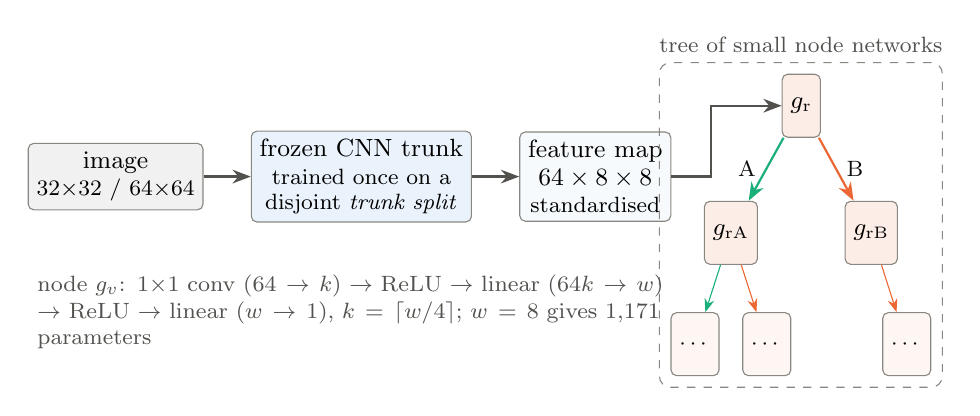
\begin{tikzpicture}[font=\small, >=Stealth, node distance=4mm,
  box/.style={draw=cMuted, rounded corners=2pt, fill=#1, minimum height=8mm, align=center, inner sep=3pt},
  box/.default=white]
  \node[box=cInkTwo!8] (img) {image\\[-1pt]{\footnotesize $32{\times}32$ / $64{\times}64$}};
  \node[box=cBlue!10, right=6mm of img] (trunk) {frozen CNN trunk\\[-1pt]{\footnotesize trained once on a}\\[-2pt]{\footnotesize disjoint \emph{trunk split}}};
  \node[box=cBlue!4, right=6mm of trunk] (feat) {feature map\\[-1pt]$64\times8\times8$\\[-1pt]{\footnotesize standardised}};
  \draw[->, thick, cInkTwo] (img) -- (trunk);
  \draw[->, thick, cInkTwo] (trunk) -- (feat);
  % tree
  \node[box=cOrange!12, right=14mm of feat, yshift=9mm] (root) {$g_{\mathrm{r}}$};
  \node[box=cOrange!12, below left=8mm and 3mm of root] (A) {$g_{\mathrm{rA}}$};
  \node[box=cOrange!12, below right=8mm and 3mm of root] (B) {$g_{\mathrm{rB}}$};
  \node[box=cOrange!6, below left=6mm and -2mm of A, font=\footnotesize] (AA) {$\cdots$};
  \node[box=cOrange!6, below right=6mm and -2mm of A, font=\footnotesize] (AB) {$\cdots$};
  \node[box=cOrange!6, below right=6mm and -2mm of B, font=\footnotesize] (BB) {$\cdots$};
  \draw[->, thick, cAqua] (root) -- node[left, font=\footnotesize, cInk] {A} (A);
  \draw[->, thick, cOrange] (root) -- node[right, font=\footnotesize, cInk] {B} (B);
  \draw[->, cAqua] (A) -- (AA);
  \draw[->, cOrange] (A) -- (AB);
  \draw[->, cOrange] (B) -- (BB);
  \draw[->, thick, cInkTwo] (feat.east) -- ++(5mm,0) |- (root.west);
  \node[draw=cMuted, dashed, rounded corners, fit=(root)(A)(B)(AA)(AB)(BB), inner sep=4pt,
        label={[font=\footnotesize, cInkTwo]above:tree of small node networks}] {};
  \node[anchor=north west, align=left, font=\footnotesize, text width=8.2cm, cInkTwo] (nodespec)
       at ($(img.south west)+(0,-7mm)$)
  {node $g_v$: $1{\times}1$ conv ($64\to k$) $\to$ ReLU $\to$ linear ($64k\to w$) $\to$ ReLU $\to$ linear ($w\to1$),
   $k=\lceil w/4\rceil$; $w=8$ gives 1{,}171 parameters};
\end{tikzpicture}
\caption{The model. A small CNN trunk, trained once on data the tree never sees, maps every image to a
$64\times8\times8$ feature map. Every node of the tree is a small neural network on that map. Child A
corrects the parent's misses and child B its false alarms.}
\label{fig:arch}
\end{figure}

\subsection{Features: one shared trunk, trained separately}
\label{sec:trunk}

Running a convolutional network inside every node would multiply the cost of the convolutions by the
number of nodes. Instead, every node reads the same frozen feature map produced by a small CNN, the
\emph{trunk}. This is the shared-trunk design proposed in Section~4.1 of the first report~\cite{saini2026tree}. The trunk
(\cref{fig:arch}) has two VGG-style stages (two $3\times3$ conv--BN--ReLU layers each, then max-pooling; a
stride-2 stem is added for the $64\times64$ Cats vs Dogs images), giving a $64\times8\times8$ map. For
pre-training only, a third stage and a linear classifier are added on top; the nodes never see them. The tap
therefore exposes \emph{mid-level} features, so the tree still has real work to do.

The key design decision is \emph{which data the trunk is trained on}. Each dataset is split into four
disjoint parts (\cref{tab:splits}). The trunk is trained only on the \emph{trunk split}, and the tree is
grown on the separate \emph{tree split}. If the trunk had seen the tree's training images, their features
would be unnaturally easy: the trunk has already memorised them (its own training accuracy is 97--99\%).
The errors that drive the tree's growth would then be unrepresentative of the errors made on new images.
This is the same reason stacked ensembles use out-of-fold predictions~\cite{wolpert1992stacked}. Three trunks are compared:
\begin{itemize}
\item \textbf{own split}: supervised on the dataset's trunk split (40 epochs, SGD, crop/flip augmentation);
\item \textbf{random}: the same architecture left untrained, with only its BatchNorm statistics calibrated, so
the tree must do all the learning;
\item \textbf{transfer} (Cats vs Dogs only): the CIFAR-10 trunk applied to images resized to $32\times32$. CIFAR-10
contains cats and dogs, but at a different resolution and from different sources.
\end{itemize}
Features are standardised per channel and cached in half precision, so a node is trained entirely on cached
tensors.

\begin{table}[t]
\centering
\small
\caption{Disjoint data splits. Cats vs Dogs is Microsoft's Kaggle release of the Asirra photos~\cite{elson2007asirra} (25{,}000 photos;
three undecodable files dropped); CIFAR-10 is from~\cite{krizhevsky2009learning}, centre-cropped and resized to $64\times64$.}
\label{tab:splits}
\begin{tabular}{@{}l r r r r r@{}}
\toprule
dataset & trunk & tree (train) & val & test & classes\\
\midrule
CIFAR-10 & 15{,}000 & 30{,}000 & 5{,}000 & 10{,}000 & 10\\
Cats vs Dogs & 6{,}000 & 11{,}997 & 2{,}000 & 5{,}000 & 2\\
\bottomrule
\end{tabular}
\end{table}

\subsection{Nodes: small neural networks}
\label{sec:node}

A node of width $w$ is the network
\[
g_v(f)=W_3\,\mathrm{ReLU}\big(W_2\,\mathrm{vec}(\mathrm{ReLU}(W_1 * f))\big),\qquad
W_1:\ 1{\times}1\text{ conv } 64\to k,\quad W_2: 64k\to w,\quad W_3: w\to1,
\]
with $k=\lceil w/4\rceil$ and biases throughout. The $1\times1$ convolution chooses which trunk channels matter,
and the linear layer over all 64 spatial positions decides \emph{where} in the image they matter. That
spatial weighting is what the receptive-field analysis of \cref{sec:rf} visualises. At the default width $w=8$
a node has 1{,}171 parameters. Nodes are trained with Adam on a class-balanced logistic loss, which gives a
good ranking even when a deep child has only a handful of positives among thousands of samples. Two further
steps follow the original LP formulation, which minimises the number of misclassified samples. After every
pass over the data, the output threshold is moved to the value that minimises the node's training errors,
never letting it become a constant. Training stops when the node makes no errors on its own sample set, or
after 20 passes without improvement.

\subsection{Growing the tree}
\label{sec:grow}

Node $v$ owns samples $S_v$ with binary targets $t_v$. After fitting $g_v$, its samples fall into the four
categories of the original paper~\cite{jayadeva2021tree}: C1 ($g=0,t=0$), C2 ($g=1,t=1$), C3 ($g=0,t=1$, misses) and C4 ($g=1,t=0$, false
alarms). Child A must turn the misses into 1s and child B the false alarms into 0s. We implement both
constructions of the children.

\paragraph{Faithful (as in the first assignment).} A is trained on \emph{all} of $S_v$, with target 1 on C3 and
0 elsewhere. B is trained on all of $S_v$, with target 1 on C4 and 0 elsewhere. The output is
$y=(g\lor A)\land\lnot B$.

\paragraph{Gated (exploiting the don't-cares).} Table~II of the paper marks A's output on C2 and B's output on
C1 as ``don't care''. In fact, under the override rule, A's output matters \emph{only} where $g=0$ and B's only
where $g=1$. We therefore train A on $\{g=0\}=C1\cup C3$ with the true targets, and B on $\{g=1\}=C2\cup C4$ with
flipped targets, and predict
\[
y(x)=\begin{cases}A(x) & \text{if } g(x)=0,\\ \lnot B(x) & \text{if } g(x)=1.\end{cases}
\]
This changes the algorithm in three useful ways.
\begin{enumerate}[(i)]
\item The children's sample sets \emph{partition} $S_v$. Each level of the tree costs one pass over the data in
total, instead of one pass per node, which was Challenge~2 of the first report.
\item A child separates its targets only from the samples the parent sent its way, not from the whole dataset.
This is an easier problem with milder class imbalance (Challenge~3).
\item Termination is immediate. A node that is not constant sends strictly fewer samples to each child, so
every path ends after at most $|S_v|$ levels, and the leaves classify their samples perfectly unless two
identical inputs carry different labels.
\end{enumerate}
Both constructions agree on how a fully grown tree classifies its training data. They differ in which subproblems
the children are asked to solve, which turns out to matter a great deal (\cref{sec:results}). A node whose sample set is pure gets a constant unit with no network. Trees are grown until every node is
error-free or a depth cap of 40 is reached.

\subsection{Multiclass: a tree of class groups}
\label{sec:hier}

For CIFAR-10 we implement the hierarchical class-grouping scheme proposed in Section~5.3 of the first
report~\cite{saini2026tree},
rather than ten one-vs-rest trees. The trunk's confusion matrix on the validation split defines a graph whose
edge weights are how often two classes are confused. We split the classes recursively along the Fiedler vector
of its normalised Laplacian~\cite{shi2000normalized,vonluxburg2007tutorial}, choosing the cut with the smallest normalised cut and requiring at least two
classes per side when possible. The 9 internal splits of the resulting binary class hierarchy are each solved
by a binary tree-type network, trained only on the samples of the classes below that split. An image is
classified by routing it down the hierarchy. Because every training image is routed correctly at every level
once every split reaches 100\% training accuracy, the whole multiclass tree then reaches 100\% training
accuracy. Classes are never compared against an unrelated jumble of other classes, and each split's tree only
has to solve the confusion that actually occurs there.

% ======================================================================
\section{Implementation}
\label{sec:impl}

Everything is implemented from scratch in PyTorch (about 1{,}800 lines) and run on an Apple M5 laptop through
the MPS (Metal) backend. The code is in the private repository linked on the first page.
\begin{itemize}
\item \texttt{treenet/trunk.py}: the trunk, its supervised training (40 epochs, SGD with Nesterov momentum,
one-cycle learning rate, weight decay $5\cdot10^{-4}$, random crop and flip), the random trunk, and feature
extraction. Training a trunk takes 2--3 minutes.
\item \texttt{treenet/tree.py}: \texttt{NodeNet}; \texttt{train\_node} (Adam, learning rate $3\cdot10^{-3}$,
batches of 512 sampled with replacement, class-balanced logistic loss, error-minimising threshold after every
pass, stop at zero errors or after 20 passes without improvement); \texttt{TreeTypeNetwork} with both child
variants, depth truncation and reduced-error pruning; and the spectral class hierarchy with
\texttt{HierarchicalTreeNetwork}.
\item \texttt{scripts/00}--\texttt{06}: data preparation, trunks, trees and baselines, double descent,
receptive fields, size minimisation, and figures. Every number and figure in this report is regenerated by
these scripts. Raw results are stored as JSON in \texttt{results/}.
\end{itemize}

\paragraph{Engineering choices that mattered.}
\begin{itemize}
\item \emph{Caching the features.} Because the trunk is frozen, its feature maps are computed once (half
precision, 0.37\,GB for CIFAR-10). Training a node is then a pass of a tiny network over a cached tensor. A
root node on all 30{,}000 CIFAR-10 tree images trains in about 15\,s, and deeper nodes, which see fewer samples, faster.
\item \emph{Class balancing and threshold calibration.} Deep children routinely face a few positives among
thousands of samples. Unweighted training then simply outputs the constant label. Balanced weighting alone
fixes that but fires on far too many negatives, which wrecked the faithful variant in our first attempt. Its
children kept creating more false alarms than they fixed, until the tree hit the depth cap. Moving the threshold
to the error-minimising value, which is the paper's own objective, fixed both problems.
\item \emph{Progress guarantee.} A node whose output is constant would hand its child the identical problem.
Such a node is retrained once with a larger learning rate and otherwise becomes a leaf. In all our runs this
only happened for sets of identical inputs with conflicting labels (\cref{sec:overfit}).
\item \emph{Disjoint splits.} The trunk, the tree, model selection and the test set use disjoint images, so
every accuracy reported is honest.
\end{itemize}


% ======================================================================
\section{Results: growing to 100\% training accuracy}
\label{sec:results}

\subsection{Overfitting is reached, and it costs test accuracy}
\label{sec:overfit}

\Cref{fig:growth} follows each tree as it grows level by level. On Cats vs Dogs the root alone, a single network of
1{,}171 parameters, already classifies 91.6\% of the training images and 88.8\% of the test images. Five more levels,
11 nodes in total (\cref{fig:tree}), take training accuracy to 99.99\% but lower test accuracy to 86.1\%. On CIFAR-10
the nine split roots together reach 82.4\% train and 71.4\% test. The full tree of 96 nodes reaches \textbf{100\%}
training accuracy at 66.7\% test. These are exactly the overfitting curves the assignment asks for: each extra node
fixes specific training images, and the fixes do not transfer.

\begin{figure}[t]
\centering
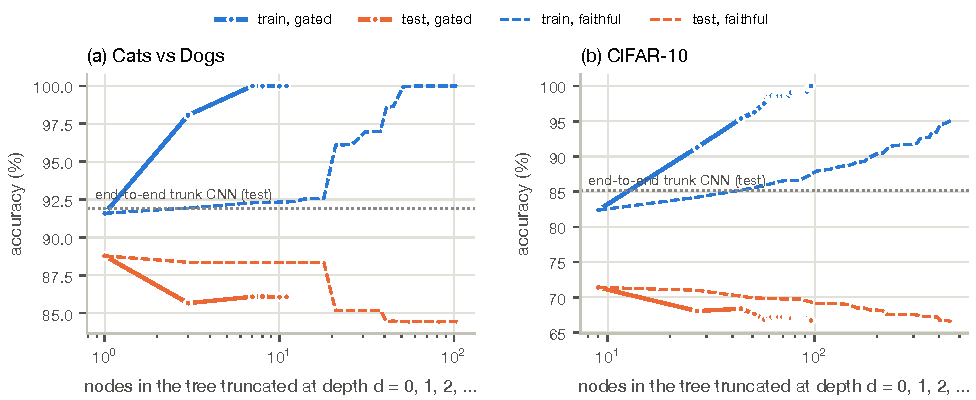
\includegraphics[width=\textwidth]{../figures/growth.pdf}
\caption{Accuracy of the tree truncated at depth $d=0,1,2,\dots$, against the number of nodes kept. Solid: gated
children; dashed: faithful children. Training accuracy climbs to 100\% while test accuracy falls; the faithful trees
need ten times more nodes to get there, and on CIFAR-10 never reach it within 40 levels.}
\label{fig:growth}
\end{figure}

\begin{figure}[t]
\centering
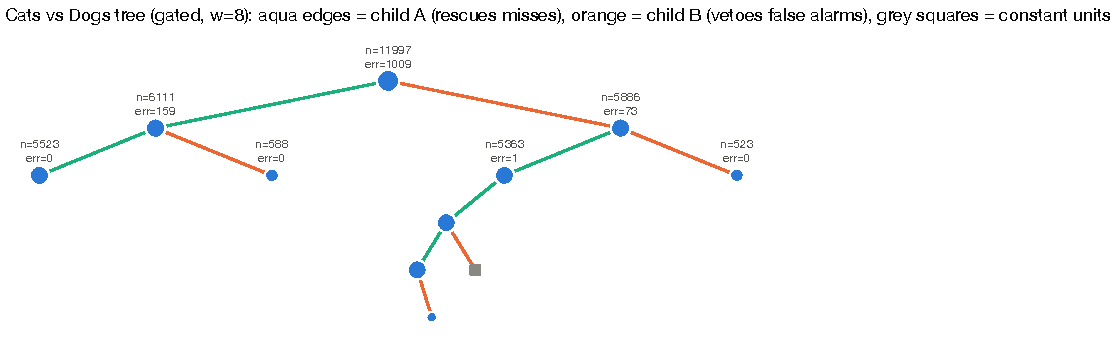
\includegraphics[width=\textwidth]{../figures/tree_catsdogs.pdf}\\[2pt]
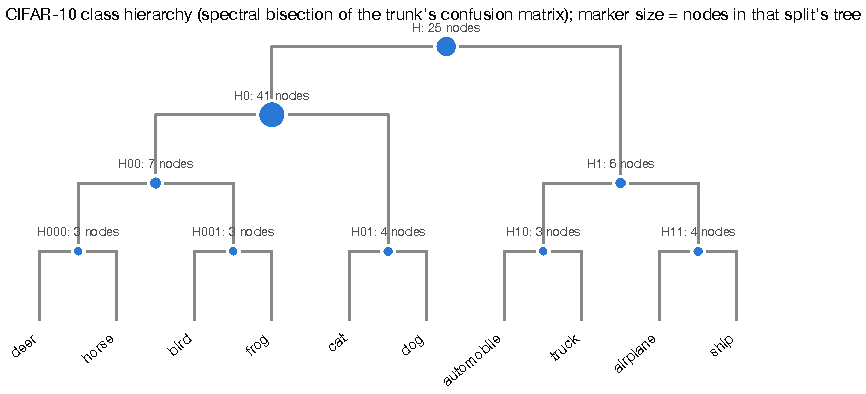
\includegraphics[width=0.92\textwidth]{../figures/hierarchy_cifar10.pdf}
\caption{Top: the grown Cats vs Dogs tree. Node size is proportional to the number of training samples it sees;
$n$ is that number and \emph{err} the node's own training errors, which its children then correct. Bottom: the
CIFAR-10 class hierarchy found by spectral bisection, with the number of nodes in each split's tree.}
\label{fig:tree}
\end{figure}

\paragraph{Why not exactly 100\% on Cats vs Dogs.} One leaf of every Cats vs Dogs tree contains three samples it
cannot separate. They are byte-for-byte identical copies of Flickr's ``photo unavailable'' placeholder, labelled dog,
dog and cat (\cref{fig:deepest}). No classifier can fit all three, so 11{,}996 of 11{,}997 is the true maximum. The
original paper asks what, besides numerical issues, can stop the error variables from all reaching zero. Duplicated
inputs with contradictory labels are a concrete answer, and the tree finds them automatically.

\paragraph{The CIFAR-10 hierarchy.} Spectral bisection of the trunk's confusion matrix recovers the natural
taxonomy: \{vehicles\} versus \{animals\}; then \{cat, dog\} versus \{deer, horse, bird, frog\}; then \{deer, horse\},
\{bird, frog\}, \{automobile, truck\} and \{airplane, ship\}. The cost of each split mirrors its difficulty. The vehicles/animals split and the split of cat and dog from the
other animals need 25 and 41 nodes and reach depths of 13 and 23. Easy pairs such as automobile versus truck need
only 3 or 4.

\paragraph{Peeling chains.} The deep CIFAR-10 nodes have a revealing structure. Along the path rA, rAA, rAAA, \dots{} of
the root split, each node receives about 17{,}900 samples, of which a few hundred are residual vehicle images (mostly
airplanes) that look like animals. Along most of the path, each node removes only one or two of them. When a small node cannot rank these
hard positives above the negatives, the error-minimising threshold isolates the single most confident one, exactly as
the paper's worked example builds a neuron that fires on one point. The tree then degenerates into a chain that
memorises one image per node. This is why the CIFAR-10 trees are deep, and why pruning removes most of them
(\cref{sec:minimize}).

\subsection{Exploiting the don't-cares: gated versus faithful children}

Both constructions classify the training data identically once fully grown, but they differ sharply in the
problems they hand to the children (\cref{tab:main}, \cref{fig:growth}). With faithful children, each child must
separate a few hundred targets from the parent's \emph{entire} sample set. Every false alarm it makes becomes a new
target for its own child B, so the trees grow into long chains. On Cats vs Dogs the result is 104 nodes reaching the
depth cap of 40, against 11 gated nodes, with lower test accuracy (84.4\% vs 86.1\%) and seven times the training
time. On CIFAR-10 the faithful tree uses 453 nodes and 530k parameters and still stops at 95.2\% training accuracy. The
gated tree reaches 100\% with 96 nodes. Treating the don't-care entries of the paper's Table~II as true don't-cares is
therefore not a detail: it is what makes the construction scale.

\subsection{Which features? Own-split, transferred and random trunks}

The trunk sets the ceiling (\cref{tab:main}). With features from a CNN trained on the dataset's own trunk split,
the Cats vs Dogs tree reaches 86.1\% test (root alone 88.8\%). The CIFAR-10 trunk transferred to Cats vs Dogs, which has
seen cats and dogs but at $32\times32$ and among eight other classes, gives 76.8\% (root 81.5\%). A random, untrained
trunk gives 62.7\% (root 66.3\%) on Cats vs Dogs and 41.7\% on CIFAR-10, where the tree also needs 163 nodes and hits the
depth cap. Weaker features mean more residual errors, so deeper trees and more memorisation. In every setting a single
node network on the same features generalises better than the grown tree, and a capacity-matched single network
better still. That a tree of small nodes trained to interpolation loses to one network of the same size is the central
negative result. \Cref{sec:dd,sec:interp} explain it.

% ======================================================================
\section{Double descent beyond the interpolation threshold}
\label{sec:dd}

To see what happens \emph{after} interpolation we need a capacity knob that can keep growing once the training set is
fitted. We use the node width $w$ (from 1 to 512, i.e.\ from 132 to 4.2M parameters per node) on a fixed subset of
4{,}000 training images, with and without 20\% symmetric label noise. For every width we grow the full gated tree,
which always interpolates, and also evaluate it truncated to the root networks alone (depth 0) and to depth~2
(\cref{fig:dd}).

\begin{figure}[t]
\centering
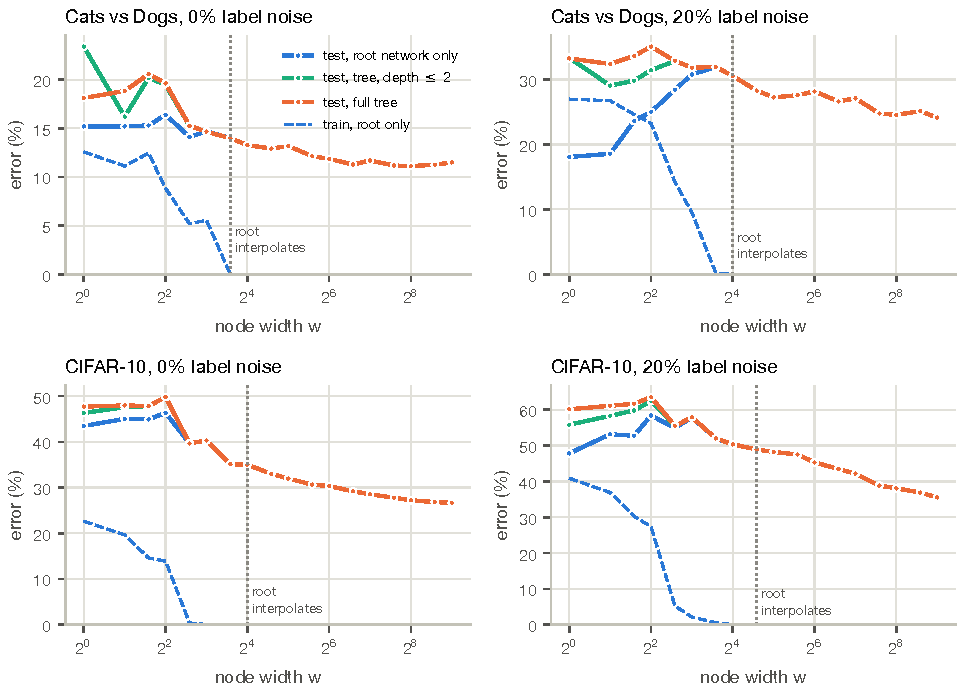
\includegraphics[width=\textwidth]{../figures/double_descent.pdf}
\caption{Test error against node width on 4{,}000 training images. Blue: the root network(s) alone; green: the tree cut
at depth 2; orange: the full tree, which always interpolates. Dashed: training error of the root. The dotted line marks
the width at which the root alone first interpolates. With label noise (right) the root's test error rises to a peak
at that threshold and descends again beyond it: double descent.}
\label{fig:dd}
\end{figure}

\begin{itemize}
\item \textbf{Double descent appears, exactly at the interpolation threshold.} With 20\% noise the root's test error on
Cats vs Dogs rises from 18.1\% ($w=1$) to a peak of 31.9\% at $w=12$, the width at which it first fits all but 0.2\% of
the noisy training labels. It then falls steadily to 24.1\% at $w=512$. That model has about 1{,}700 times more parameters than needed to
interpolate, and it is \emph{better} than the model at the threshold. CIFAR-10 shows the same shape: 47.8\%,
then a peak of 58\% near the threshold ($w=4$--$8$), then down to 35.5\%. Without noise the peak shrinks to a small
bump (Cats vs Dogs 15.2\%$\to$16.4\%$\to$11.1\%; CIFAR-10 43.5\%$\to$46.3\%$\to$26.7\%), as the literature
predicts~\cite{belkin2019reconciling,nakkiran2020deep}.
\item \textbf{Interpolating with many tiny nodes is the worst way to interpolate.} Below the threshold a single node
cannot fit the data, so the tree adds nodes until it does. These trees always interpolate, yet their test error is the
highest in the plot: 32--35\% on noisy Cats vs Dogs and 60--64\% on noisy CIFAR-10. That is worse than both the
non-interpolating root and the wide interpolating node. Beyond the threshold the root interpolates alone, the tree
collapses to that single node, and the curves coincide.
\item \textbf{Reading.} In the tree, interpolation is reached by \emph{partitioning}: each correction node carves out
a small region around the training points its parent got wrong, and a mislabelled point gets a region of its own. A
wide single network interpolates by fitting a smooth function through all points at once, and the implicit bias of
gradient training towards small-norm solutions spreads the damage of each noisy label thinly. The second descent is
that bias growing with width. The tree's hard, local corrections cannot benefit from it.
\end{itemize}

% ======================================================================
\section{Receptive fields of the nodes}
\label{sec:rf}

For every node we route the training images through the tree to recover the node's own sample set. We then compute
three views (\cref{fig:rf-cd,fig:rf-c10}):
\begin{itemize}
\item \textbf{Mean Grad-CAM}~\cite{selvaraju2017gradcam} at the $8\times8$ trunk feature map, over the images the node
fires on: \emph{where} in the image its decision comes from.
\item \textbf{Activation maximisation}~\cite{erhan2009visualizing,olah2017feature}: an input optimised through the
frozen trunk to maximise the node's output, regularised by jitter, $\ell_2$ and total variation. This shows
\emph{what} the node looks for.
\item \textbf{The node's most strongly activating training images}, darkened where Grad-CAM is low.
\end{itemize}

\begin{figure}[p]
\centering
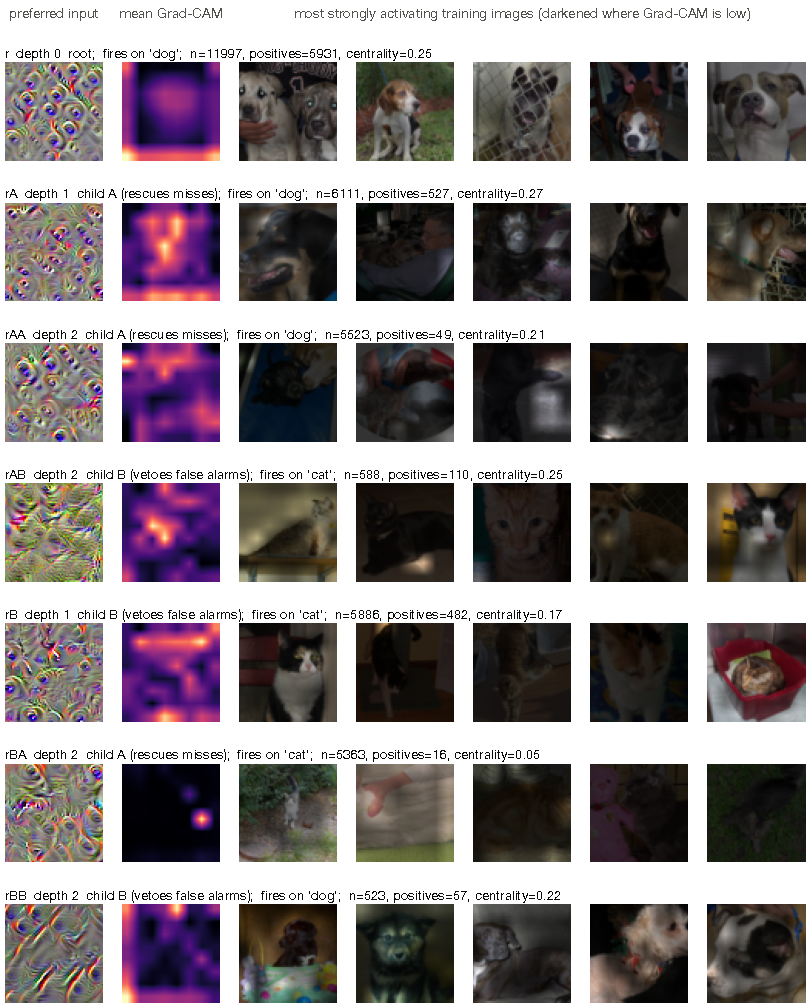
\includegraphics[width=0.88\textwidth]{../figures/rf_catsdogs.pdf}
\caption{Receptive fields of the Cats vs Dogs tree (all nodes up to depth 2). ``Fires on'' names the class the node's
output~1 stands for. Centrality is the share of Grad-CAM mass in the central $4\times4$ of the $8\times8$ grid
(uniform = 0.25).}
\label{fig:rf-cd}
\end{figure}

\begin{figure}[p]
\centering
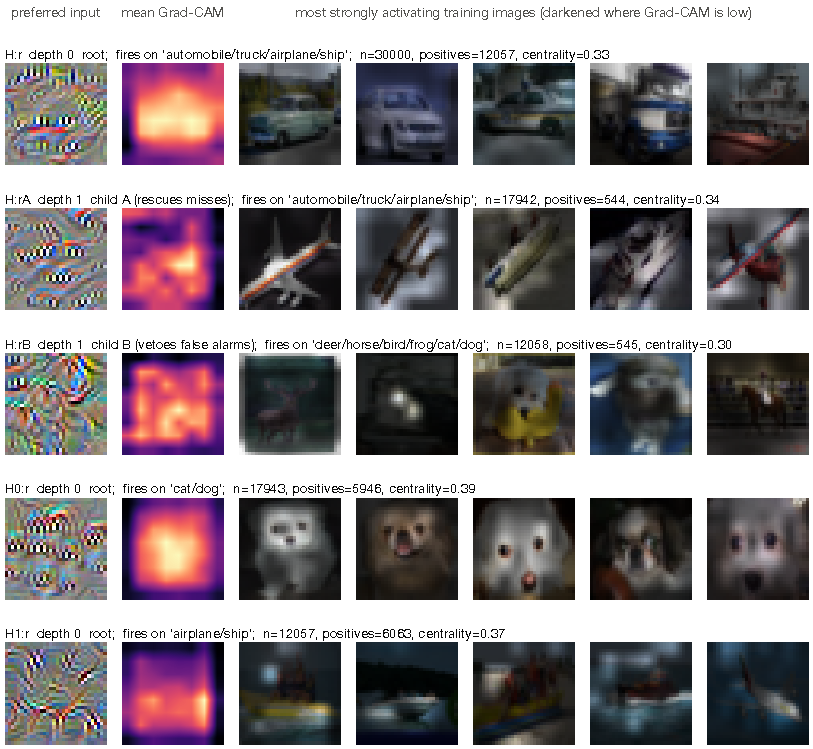
\includegraphics[width=0.88\textwidth]{../figures/rf_cifar10.pdf}
\caption{Receptive fields in the CIFAR-10 tree: the root of the vehicles/animals split and its two children, and the
roots of the cat-and-dog split (H0) and the airplane-and-ship split (H1).}
\label{fig:rf-c10}
\end{figure}

\paragraph{Observations.}
\begin{enumerate}[(1)]
\item \textbf{Roots learn the class.} The Cats vs Dogs root responds to dog faces: its preferred input is tiled with
eye-like blobs and fur texture, and its top images are frontal dog faces. On CIFAR-10 the root of the cat-and-dog
split (H0) attends to faces and eyes (centrality 0.39). The vehicles root responds to car and truck bodies.
\item \textbf{Correction children specialise in the parent's blind spots.} On CIFAR-10, child A of the root, which
rescues vehicles mistaken for animals, fires almost only on \emph{airplanes}: diagonal shapes on a plain background,
easily mistaken for birds. Child B, which vetoes animals mistaken for vehicles, fires on animals in boxy or
man-made surroundings: a horse behind a fence, a dog in a crate. On Cats vs Dogs the misses rescued by child A are
dark, low-contrast photos, and the deepest nodes respond to a single small spot (node rBA, centrality 0.05).
\item \textbf{Shortcuts.} The root of the airplane/ship versus automobile/truck split (H1) fires on blue sky and
water. Its Grad-CAM covers the background, not the object, a textbook shortcut~\cite{geirhos2020shortcut}. It is
correct on the training set, which is why the tree has no reason to fix it.
\item \textbf{Attention leaves the object as depth grows} (\cref{fig:centrality}). The median share of Grad-CAM mass on
the central quarter of the image falls from 0.37 at the CIFAR-10 roots to 0.29, 0.27, 0.25 and 0.21 at depths 1, 2, 3--5
and beyond 5; on Cats vs Dogs it falls from 0.25 to 0.21. Deep nodes increasingly decide from the periphery: background,
context and image borders. This is what memorising a handful of specific images looks like.
\end{enumerate}

\begin{figure}[t]
\centering
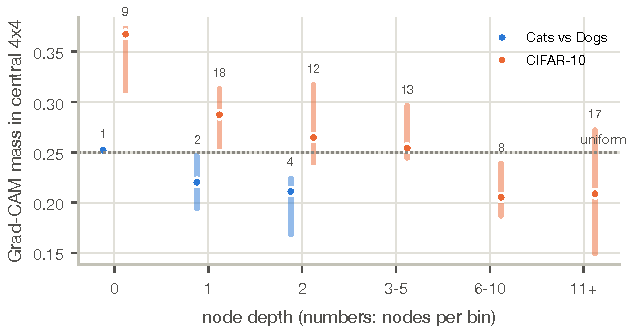
\includegraphics[width=0.62\textwidth]{../figures/rf_centrality.pdf}
\caption{Share of Grad-CAM mass in the central quarter of the image, by node depth (dot: median; bar: interquartile
range; numbers: nodes).}
\label{fig:centrality}
\end{figure}

\begin{figure}[t]
\centering
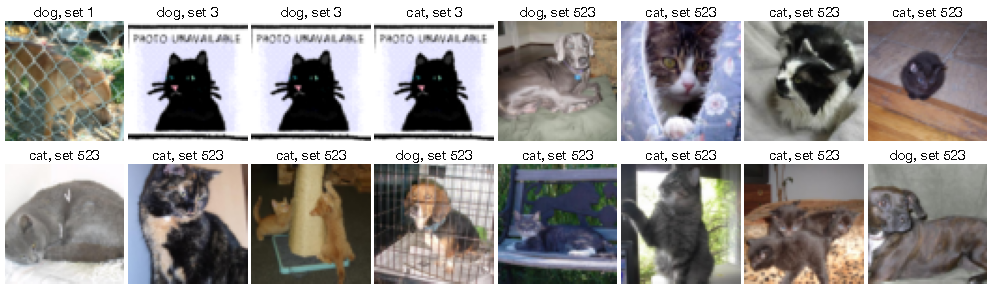
\includegraphics[width=\textwidth]{../figures/deepest_catsdogs.pdf}
\caption{Training images of Cats vs Dogs that end in the smallest final sets of the tree (``set'' = size of the final
node's sample set). The three copies of Flickr's placeholder carry contradictory labels and form the only unfittable
leaf.}
\label{fig:deepest}
\end{figure}

% ======================================================================
\section{Minimising the size of the network}
\label{sec:minimize}

The network is the shared trunk plus the tree. The trunk is paid for once: 65.8k parameters up to the feature
map for CIFAR-10, 75.0k for Cats vs Dogs. We therefore minimise the tree, using three levers (\cref{tab:minimize,fig:minimize}).

\begin{table}[t]
\centering
\small
\caption{Shrinking the tree. ``Non-zero'' counts weights left after magnitude pruning inside the nodes.}
\label{tab:minimize}
\setlength{\tabcolsep}{4.5pt}
\begin{tabular}{@{}l l r r r r r@{}}
\toprule
dataset & model & nodes & node parameters & non-zero & train (\%) & test (\%)\\
\midrule
Cats vs Dogs & full tree, $w=8$ & 11 & 11{,}711 & 11{,}711 & 99.99 & 86.1\\
 & smallest interpolating tree, $w=1$ & 91 & 11{,}488 & 11{,}488 & 99.99 & 82.1\\
 & $w=8$ + magnitude pruning inside nodes & 11 & 11{,}710 & 8{,}602 & 99.99 & 86.1\\
 & $w=8$ + reduced-error pruning & 1 & 1{,}171 & 1{,}171 & 91.59 & 88.8\\
\addlinespace
CIFAR-10 & full tree, $w=8$ & 96 & 110{,}076 & 110{,}076 & 100 & 66.7\\
 & smallest interpolating tree, $w=16$ & 14 & 61{,}446 & 61{,}446 & 100 & 70.7\\
 & $w=8$ + magnitude pruning inside nodes & 96 & 110{,}074 & 68{,}100 & 100 & 66.8\\
 & $w=8$ + reduced-error pruning & 13 & 15{,}223 & 15{,}223 & 83.30 & 71.4\\
\bottomrule
\end{tabular}

\end{table}

\begin{figure}[t]
\centering
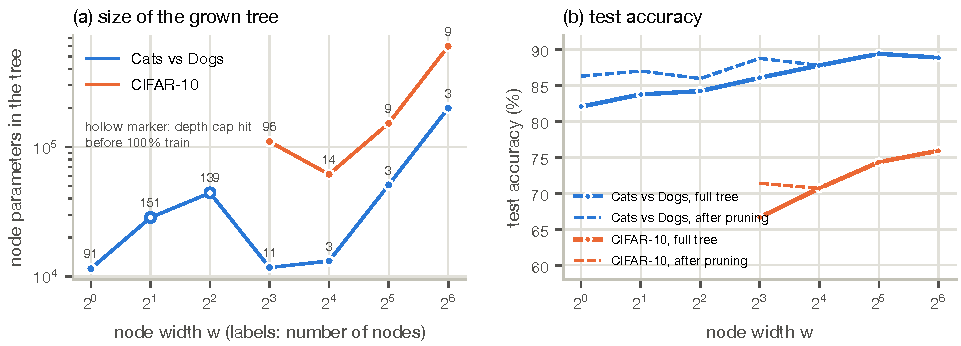
\includegraphics[width=\textwidth]{../figures/minimize.pdf}
\caption{Growing the full tree with nodes of different widths. (a) Total node parameters; labels give the number of
nodes. (b) Test accuracy of the grown tree (solid) and after validation pruning (dashed).}
\label{fig:minimize}
\end{figure}

\begin{enumerate}[(1)]
\item \textbf{Choose the node width.} Size is not monotone in width. Very small nodes need many of themselves: 91
nodes at $w=1$ on Cats vs Dogs, and at $w=2$ and $w=4$ the trees grow peeling chains to the depth cap before they
interpolate. Very wide nodes waste parameters. The smallest tree that still fits the data has about 11.5k node
parameters on Cats vs Dogs, whether as 91 one-unit nodes or 11 width-8 nodes. On CIFAR-10, width 16 needs only 14 nodes
and 61k parameters, against 96 nodes and 110k at width 8, and is more accurate (70.7\% vs 66.7\%). A slightly wider
node avoids the peeling chains altogether.
\item \textbf{Prune weights inside the nodes.} We prune each node's weights by magnitude, at increasing sparsity, with
a short masked fine-tune that must reproduce the node's \emph{own decisions on its own training set exactly}, so the
tree's training predictions cannot change~\cite{han2015learning,frankle2019lottery}. This deletes 26.5\% of the node
weights on Cats vs Dogs and 38.1\% on CIFAR-10. Training accuracy is unchanged and test accuracy is unchanged or
slightly higher. The savings are very uneven. About half the nodes cannot lose any weight without changing a
decision, while a dozen CIFAR-10 nodes keep less than 10\% of theirs.
\item \textbf{Prune subtrees on validation data.} Bottom-up reduced-error pruning~\cite{quinlan1987simplifying}
replaces a subtree by its root whenever that does not hurt accuracy on the validation images reaching it. Cats vs
Dogs collapses to the single root node: 1{,}171 parameters, $10\times$ smaller, with test accuracy \emph{up} from 86.1\% to
88.8\%. CIFAR-10 keeps 13 of 96 nodes: $7\times$ smaller, test up from 66.7\% to 71.4\%. Here minimising size and
improving generalisation are the same operation. It gives up 100\% training accuracy, which is the point.
\end{enumerate}

% ======================================================================
\section{Extra: the tree as a detector of mislabelled examples}
\label{sec:noise}

If the corrections are local, a mislabelled image should end up isolated: the tree must carve it out of a region full
of correctly labelled neighbours. We tested this by flipping 20\% of the labels of a 4{,}000-image subset, growing the
tree, and scoring each training image by the size of the final node set it lands in, where smaller means more
suspicious (\cref{fig:noise}). With width-2 nodes this finds the flipped labels with ROC-AUC 0.66 on Cats vs Dogs and
0.74 on CIFAR-10. Among the 793 most suspicious images, 36\% and 43\% are flipped, against a base rate of 20\%. Flipped
images end in sets about three times smaller (median 373 vs 1{,}284, and 133 vs 408). Two negative findings are just as
informative. The \emph{depth} at which an image is resolved carries no signal (AUC 0.40 and 0.49): mislabelled images
are peeled off early into tiny sets, while their clean neighbours continue down the chain. And with width-8 nodes the
detector fails (AUC 0.37 and 0.48), because a single width-8 node is large enough to memorise most flipped labels on
4{,}000 images before the tree ever has to isolate them. The tree is a useful noise detector only in the regime of
the original construction, where nodes are too weak to memorise. On the real Cats vs Dogs data, the smallest final sets
are exactly the placeholder images and an outlier photo (\cref{fig:deepest}). This complements dedicated tools such as
confident learning~\cite{northcutt2021confident}.

\begin{figure}[t]
\centering
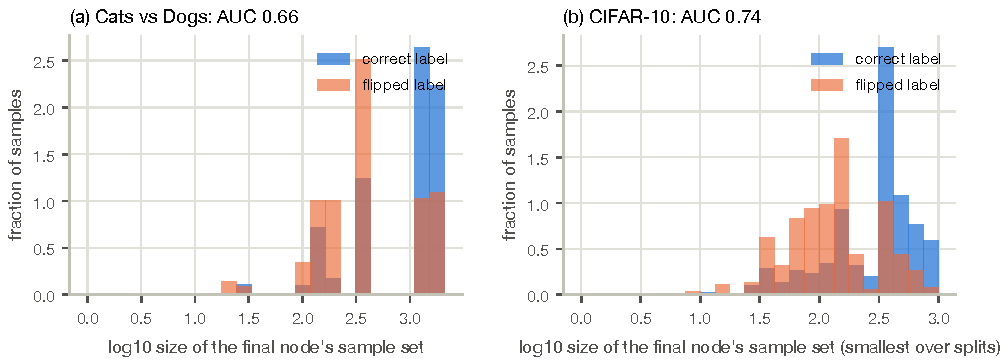
\includegraphics[width=\textwidth]{../figures/noise_detection_w2.pdf}
\caption{Size of the final node set for clean and deliberately flipped training labels (width-2 nodes, 20\% noise,
4{,}000 images). Flipped labels end in much smaller sets.}
\label{fig:noise}
\end{figure}

% ======================================================================
\section{Interpretations and conclusions}
\label{sec:interp}

\begin{enumerate}[(1)]
\item \textbf{The construction works at scale once nodes are networks on shared features.} A frozen trunk, trained on
data the tree never sees, plus nodes of about 1k parameters, grows trees that interpolate 30{,}000 CIFAR-10 images in
about half an hour on a laptop. Per-node cost is negligible because the convolutional work is done once.
\item \textbf{Respect the don't-cares.} Training each child only where its output can change the answer turns the tree
into a partition of the data. It cuts the size by 4--10$\times$, removes the chains that grow when children must
separate their targets from everything, and improves test accuracy. Calibrating each node's threshold to minimise
errors, the paper's own objective, is what made deep, very unbalanced children trainable.
\item \textbf{Interpolation is reached by memorising, and memorising has a recognisable signature.} Deep nodes see
few positives, attend to the image periphery rather than the object, respond to single images, backgrounds and
dataset artefacts, and can be pruned away with a gain in test accuracy. The tree's growth curve is the classical
overfitting curve, and its growth to 100\% is its least useful phase.
\item \textbf{Double descent is a property of how a model interpolates, not just whether it does.} A single wide node
that interpolates generalises better and better with width. A tree that interpolates with many small, local
corrections does not, because each correction is effectively a lookup for a few training points. This is the same
mechanism by which networks can fit random labels~\cite{zhang2017understanding} while still learning simple patterns
first~\cite{arpit2017closer}. A tree makes the memorisation explicit and inspectable: it is the deep nodes.
\item \textbf{Size and generalisation can be optimised together.} The smallest good tree is not the smallest
interpolating tree but the pruned one: one node on Cats vs Dogs, 13 on CIFAR-10. This echoes the course's theme that
fewer effective degrees of freedom generalise better, and the motivation of the Minimal Complexity
Machine~\cite{jayadeva2015learning}.
\end{enumerate}

% ======================================================================
\section{Future directions}
\label{sec:future}

\begin{itemize}
\item \textbf{Validation-gated growth.} Stop expanding a node as soon as its children do not help on held-out data.
This grows the pruned tree directly and saves training the nodes that are later removed.
\item \textbf{Progress-aware thresholds.} Replace the pure error-minimising threshold with one that requires each
node to fire on a minimum fraction of its targets. This would cut the peeling chains of \cref{sec:overfit}, trading a
few more errors per node for much shallower trees.
\item \textbf{Specialist trunks per class group.} Train a small trunk for each split of the CIFAR-10 hierarchy, for
example one for the confusable animal splits, instead of one shared trunk. This is a ``set of trunks trained
separately'' in the assignment's sense.
\item \textbf{Soft routing and end-to-end fine-tuning.} Make the override differentiable and fine-tune the trunk
through the tree. This connects to neural decision trees and forests~\cite{kontschieder2015deep,tanno2019adaptive}
and to hierarchical mixtures of experts~\cite{jordan1994hierarchical}.
\item \textbf{Minimal-complexity nodes.} Train each node with the MCM objective~\cite{jayadeva2015learning}, which
directly minimises a bound on its VC dimension, so that every correction is as simple as the data allow.
\item \textbf{Distillation in both directions.} Distil the tree into one compact network, or a network into a
tree~\cite{frosst2017distilling} for interpretability. Separately, use the tree's tiny leaves as a cheap
dataset-cleaning tool on larger, noisier datasets.
\end{itemize}

\small
\bibliographystyle{unsrtnat}
\bibliography{refs}

\end{document}
